\section{Music Recognizer}

Для лучшего тестирования было разработано веб-приложение, структурная схема
которого представлена на Диаграмме \ref{F:6-sd}. Исходный код
веб-приложения, графиков, отчёта и презентации доступен по ссылкам
\cite{L:course-paper}, \cite{L:music-recognizer}.

\begin{figure}[b]
  \centering
  \begin{tikzpicture}[every node/.style=draw]
    \matrix [matrix of nodes, column sep=5mm, row sep=5mm]
    {
      \node[align=center](a) { Микрофон\\ pyaudio}; & \\
      \node[align=center](b) { WAV файл\\ sms-tools}; &
          \node[align=center](d) {Обработка\\ аудио сигнала\\ pitch-estimator.py};
          & \node[align=center](e)
          {Определение\\ фундаментальной частоты\\ Online-STFT.py}; \\
      \node[align=center](c)
          {Удалённый микрофон\\ (NodeJS, WebSockets,\\ WebAudioAPI)};
          & \node[align=center](f) {Генерация аннотации\\ в build/twm.txt};
          & \node[align=center](g) {Запись аудио сигнала\\ в build/output.wav}; \\
    };

    \draw [line width=0.3mm, ->] (a) -- (d);
    \draw [line width=0.3mm, ->] (b) -- (d);
    \draw [line width=0.3mm, ->] (c) -- (d);
    \draw [line width=0.3mm, ->] (d) -- (e);
    \draw [line width=0.3mm, ->] (e) -- (f);
    \draw [line width=0.3mm, ->] (e) -- (g);

  \end{tikzpicture}
  \caption{Структурная диаграмма}
    \label{F:6-sd}
\end{figure}

\subsection{Определение фундаментальной частоты используя \\
процедуру two-way mismatch}

Определение фундаментальной частоты в квазигармонических сигналах
является важной задачей в обработке музыкальных сигналов.
Процедура \textit{RCMJW} (TWM) определения $F_0$ -
это компьютерный метод, который опирается на квазигармоничность,
что позволяет находить $F_0$ на основе кратковременного спектра входного
сигнала.
Найденная $F_0$ выбирается так, что минимизируется расхождение между
измеренными частотными (синусоидальными) компонентами и гармоническими
компонентами сгенерированными на основе текущего кандидата для $F_0$.
Для каждой пробы $F_0$, несовпадения между сгенерированными гармониками
и измеренными частотными компонентами усредняются на фиксированном
подмножестве доступных компонент. Схема взвешивания используется для
снижения чувствительности процедуры к наличию шума или отсутствию
определенных компонент в спетральных данных.

Алгоритм основан на определении синусоидальных компонент с помощью STFT.
После этого для каждого окна определяется множество $F_0$ и как результат
выбирается та, у которой минимальная ошибка.

Процедура использует следующие функции ошибки:
\begin{align}
  Err_{p \to m} &= \sum_{n=1}^N E_\omega (\Delta f_n, f_n, a_n, A_{max}) \\
                &= \sum_{n=1}^N \Delta f_n \times (f_n) ^{-p} +
                       (\frac{a_n}{A_{max}}) \times [q \Delta f_n \times
                       (f_n)^{-p} - r],
\end{align}

где $\Delta f_n$ есть разница между предсказанными и наиближайшеми измеренными
пиками, $f_n, a_n$ есть частота и магнитуда предсказанных пиков,
$A_{max}$ есть максимальная магнитуда среди пиков.

\begin{align}
  Err_{m \to p} &= \sum_{k=1}^K E_\omega (\Delta f_k, f_k, a_k, A_{max}) \\
                &= \sum_{k=1}^K \Delta f_k \times (f_k) ^{-p} +
                       (\frac{a_k}{A_{max}}) \times [q \Delta f_k \times
                       (f_k)^{-p} - r],
\end{align}

где $\Delta f_k$ есть разница между измеренными и наиближайшеми предсказанными
пиками, $f_k, a_k$ есть частота и магнитуда измеренных пиков,
$A_{max}$ есть максимальная магнитуда среди пиков.

\textbf{Суммарная ошибка:} $Err_{total} = Err_{p \to m}/N + \rho Err_{m \to p}/K$.

Maher и Beauchamp предлагают следующие значения для параметров
$p=0.5, q=1.4, r=0.5, \rho=0.33$.

\subsection{Демонстрация}

В системе используется реализация TWM из \cite{L:sms-tools}.

Входной сигнал может поступать из:
\begin{enumerate}
  \item WAV аудио файла, Диаграмма \ref{F:6-2-t-y-a-f};
  \item Комьютерного микрофона;
  \item Микрофон браузера с клиента через веб-приложение,
      Диаграмма \ref{F:6-2-t-y-a-m}.
\end{enumerate}

Для тестирования была использована аудиозапись \cite{L:daj-ci-boza}.

\begin{figure}
  \centering
    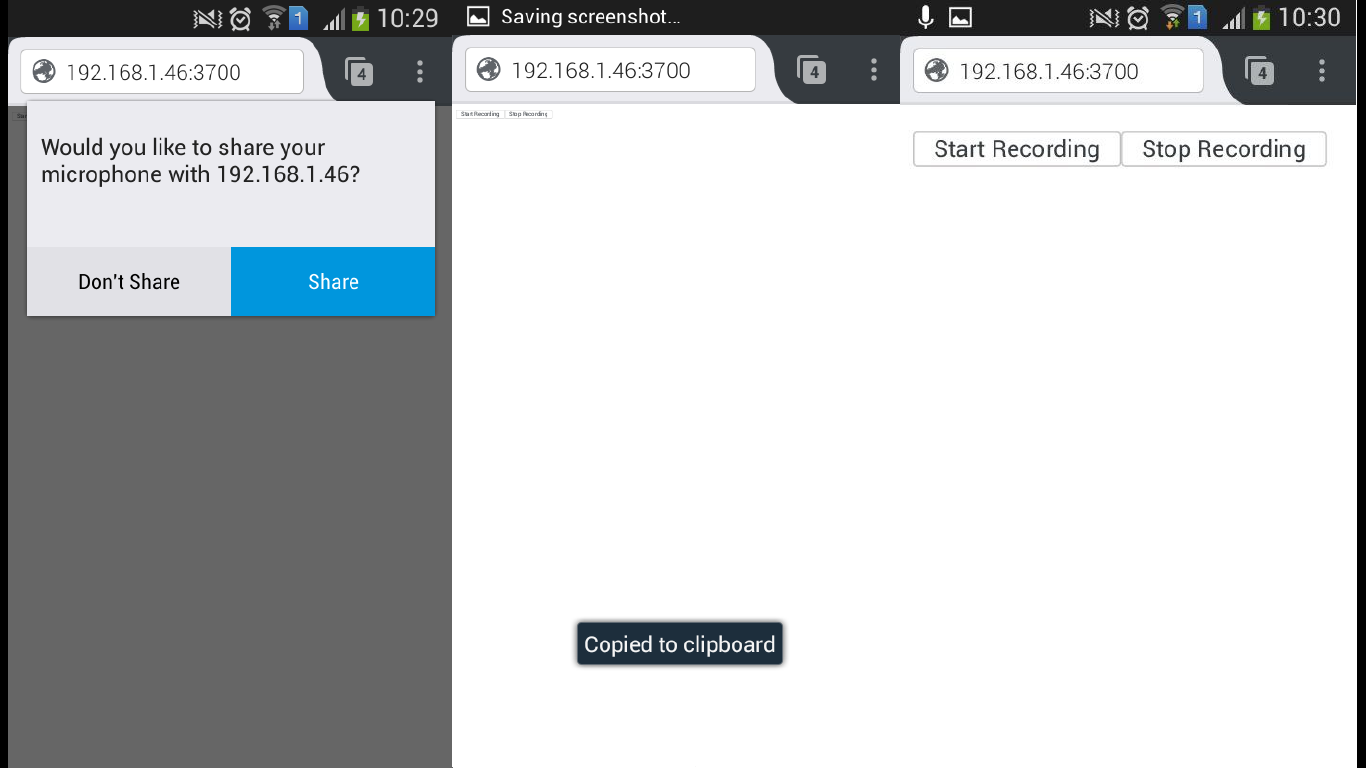
\includegraphics[scale=.25]{res/android-firefox-music-recognizer.png}
  \centering
  \caption{Скриншот веб-приложения с Android браузера}
    \label{F:6-2-afmr}
\end{figure}

\begin{figure}
  \centering
    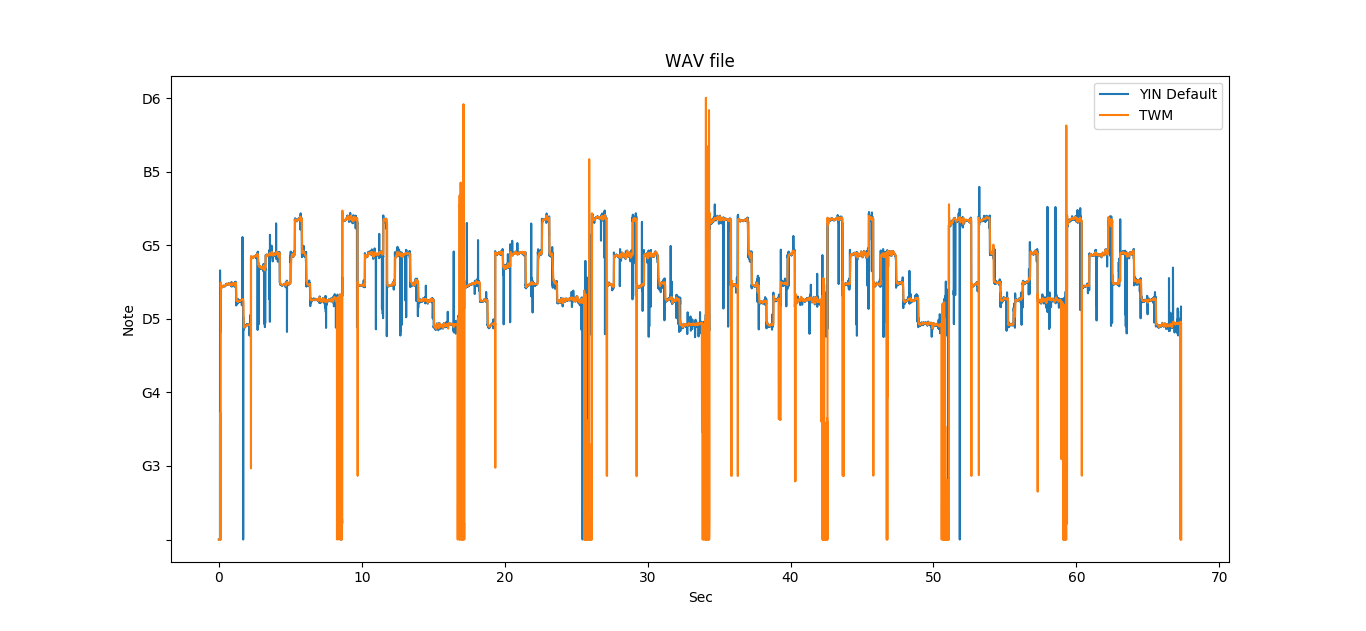
\includegraphics[scale=.5]{res/daj-ci-boze-dobranoc-twm-vs-yin.png}
  \centering
  \caption{WAV аудио запись.
    Сравнительная аннотация фундаментальной частоты процедуры
    TWM с потоковым алгоритмом YIN из Aubio.
    (Текущая реализация NMF не позволяет применение
    к потоковой обработке и тем более к определению фундаментальной
    частоты}
    \label{F:6-2-t-y-a-f}
\end{figure}

\begin{figure}
  \centering
    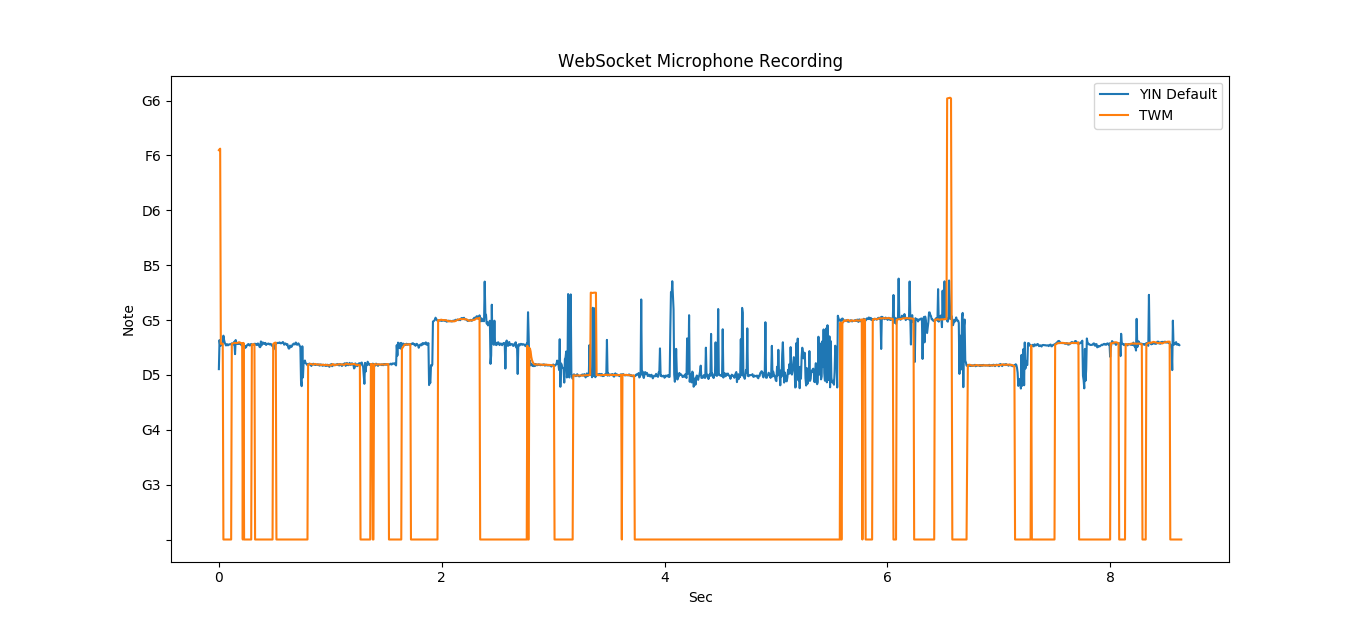
\includegraphics[scale=.5]{res/record-twm-vs-yin.png}
  \centering
  \caption{Удалённый микрофон, запись.
    Сравнительная аннотация фундаментальной частоты процедуры
    TWM с потоковым алгоритмом YIN из Aubio.
    (Текущая реализация NMF не позволяет применение
    к потоковой обработке и тем более к определению фундаментальной
    частоты}
    \label{F:6-2-t-y-a-m}
\end{figure}

\subsection{Существующие библиотеки для решения задачи}

До этого момента разработка алгоритмов производилась на языке Octave.
Который представляет собой бесплатную альтернативу MATLAB, но имеет
менее богатую библиотеку расширений.

Для дальнейшей работы было решено переходить на python библиотеки,
так как все современный библиотеки ориентируются на эту платформу.

Приложения для автоматической транскрипции музыки должно опираться
на библиотеку для обработки аудио сигналов. Среди доступных в интернете
были выделены следующие разработки:
\begin{enumerate}
  \item Essentia, содержит огромное количество классических алгоритмов
    для аудио обработки, имеет как потоковый, так и оффлайновый режимы
    обработки
  \item Aubio, кроссплатформенная библиотека, достаточно портативная,
    содержит реализацию YIN алгоритма
  \item librosa, набор утилит для работы с аудио сигналами, удобно
    для прототипирования, аналог Octave и MATLAB библиотек
  \item madmom, очередная библиотека с алгоритмами для обработки
    аудио сигналов, имеет базовую архитектуру для алгоритмов на базе
    машинного обучения
\end{enumerate}

\subsection{Направления для дальнейшей работы}

У проделанной работы есть очень важный недостаток, почти
все алгоритмы были рассмотрены в рамках нескольких примеров.
Не было проведено никакого статистического оценивания работы
алгоритмов. Для этих целей следует разработать систему автоматического
тестирования.

Среди последних исследований можно выделить работу \cite{SBETENN}.

Авторы строят гибридную нейронную сеть для автоматической транскрипции
полифноческих музыкальных композиций. Для оценки работы системы
используется датасет MAPS \cite{L:MAPS}. Но полученная точность $\approx 70\%$
не превышает подобную у более классических алгоритмов.
В статье указывают на главную проблему - не большой размер датасета.

Для ознакомления с этими исследованиями и продолжения работу дальнейшей работы
по напровлению распознавания нотных последовательностей стоит воспользоваться
реализацией нейронной сети со схожей архитектурой
\cite{KCFGAMT}, \cite{L:auto-music-tagger}.
